\documentclass[11pt, a4paper]{article}

% Basic packages
\usepackage{amsmath,amssymb,amsfonts}
\usepackage{bm,ltablex,microtype}
\usepackage[pdftex]{graphicx}
\usepackage[utf8]{inputenc}
\usepackage{parskip}
\usepackage[section]{placeins}
\usepackage[table,xcdraw]{xcolor}
%\usepackage[capitalise, noabbrev]{cleveref} Discarded in favor of hyperref
\definecolor{linkcolor}{rgb}{0,0,0.4}

\usepackage{fancyvrb}
\usepackage{csvsimple}
\usepackage{booktabs}
\usepackage{multicol}
\usepackage[margin=3cm]{geometry}

\usepackage{listings}
\lstset{
    language=Python,
    inputencoding=utf8,
    extendedchars=true,
    literate={ø}{{\o}}1 {å}{{\r a}}1 {Å}{{\r A}}1 {æ}{{\ae}}1,
    backgroundcolor=\color{white!88!black},
    basicstyle=\footnotesize\ttfamily,
    breakatwhitespace=false,
    breaklines=true,
    captionpos=b,
    commentstyle=\itshape\color{purple!60!black},
    frame=single,
    %identifierstyle=\color{orange},
    keepspaces=true,
    keywordstyle=\bfseries\color{violet},
    numbers=left,
    numbersep=5pt,
    numberstyle=\tiny\color{black},
    rulecolor=\color{black},
    showstringspaces=false,
    showtabs=false,
    stepnumber=1,
    stringstyle=\color{purple!60!black},
    tabsize=2,
    title=\lstname
  }
%\usepackage{tikz}
%\usetikzlibrary{math,calc,positioning}

%\usepackage{todonotes}

\usepackage{hyperref}
\hypersetup{
    breaklinks=true,
    colorlinks=true,
    linkcolor=black,
    urlcolor=linkcolor,
    citecolor=black,
    filecolor=black,
    %filecolor=blue,
    pdfmenubar=true,
    pdftoolbar=true,
    bookmarksdepth=3   % Uncomment (and tweak) for PDF bookmarks with more levels than the TOC
    }

% Set up fonts
% \usepackage{fontspec}
% \usepackage{unicode-math}
% \setmainfont{STIX Two Text}
% \setmathfont{STIX Two Math}

\title{FYS-STK4155 - Project1}
\author{Gard, Are, David Andreas Bordvik}
\date{\today}

\begin{document}

\maketitle
  
\section*{Motivation}
In Project 1, we are tasked to study various regressions methods, such as Ordinary Least Squares, Ridge and Lasso. Our first area of study is how to fit polynomials to a specific two-dimensional function called Franke's Function. Our motivation behind fitting polynomials to Frank's function is to test the implementation of our regression algorithms, as well as studying various techniques such as bootstrapping and measurements such as the bias-variance tradeoff. Finally, we will move on to use real digital terrain data for our analysis.

The Franke Function is given on the form

\begin{align*}
  f(x,y) &= \frac{3}{4}\exp{\left(-\frac{(9x-2)^2}{4} - \frac{(9y-2)^2}{4}\right)}+\frac{3}{4}\exp{\left(-\frac{(9x+1)^2}{49}- \frac{(9y+1)}{10}\right)} \\
  &+\frac{1}{2}\exp{\left(-\frac{(9x-7)^2}{4} - \frac{(9y-3)^2}{4}\right)} -\frac{1}{5}\exp{\left(-(9x-4)^2 - (9y-7)^2\right) }
\end{align*}

with a 3-dimensional plot given in Figure \ref{fig:1}

\begin{figure}[h]
  \centering
  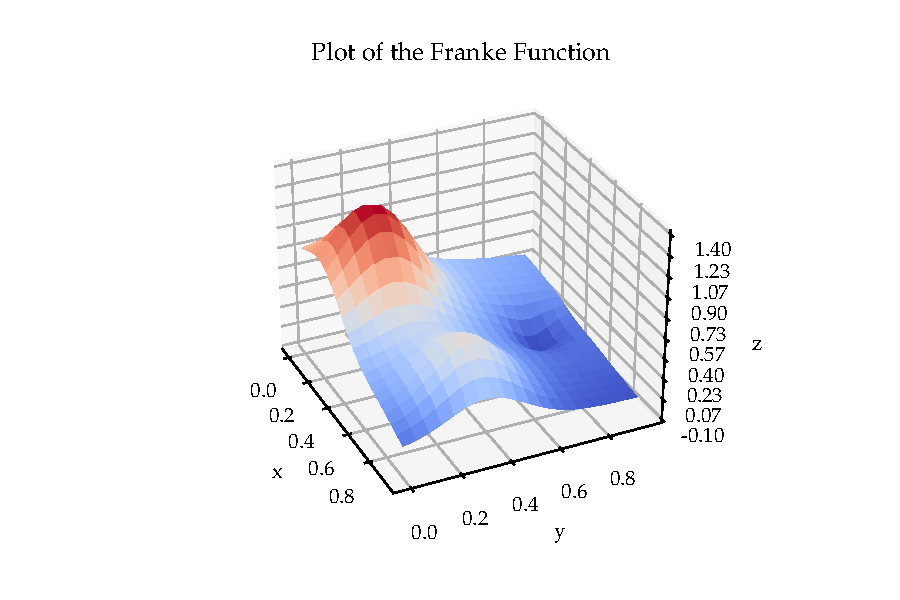
\includegraphics[scale=0.75]{figures/EX1_franke_function_nonoise_preview.pdf}
  \caption{\label{fig:1}Plot of the Franke Function}
\end{figure}

\section*{Theory}
The sample mean value of $\boldsymbol{y}$ is defined as;
\begin{equation}
    \bar{y} =  \frac{1}{n} \sum_{i=0}^{n - 1} y_i
\end{equation}

The sample variance of $\boldsymbol{y}$ is defined as;
\begin{equation}
    \mathrm{var}[\boldsymbol{x}]=\frac{1}{n}\sum_{i=0}^{n-1}(x_i- \overline{x})^2=\mathbb{E}\left[(\bm{y}-\bm{\tilde{y}})^2\right]
\end{equation}

\section*{Exercise 1}
In Machine Learning, we are studying the problem of optimization, that is, finding the optimal parameter $\beta$ such that $C(\boldsymbol{X},\boldsymbol{\beta}) = 
{\displaystyle \min_{\boldsymbol{\beta}\in {\mathbb{R}}^{p}}}\frac{1}{n}\left\{\left(\boldsymbol{y}-\boldsymbol{X}\boldsymbol{\beta}\right)^T\left(\boldsymbol{y}-\boldsymbol{X}\boldsymbol{\beta}\right)\right\}
$ our cost function is minimized. For the following exercise, where we will study Ordinary Least Squares regression, the previously stated cost function is the one we will minimize in order to fit the Franke Function, both without (as in Figure (\ref{fig:1})) and with noise as in Figure (\ref{fig:2}). 

\begin{figure}[h]
  \centering
  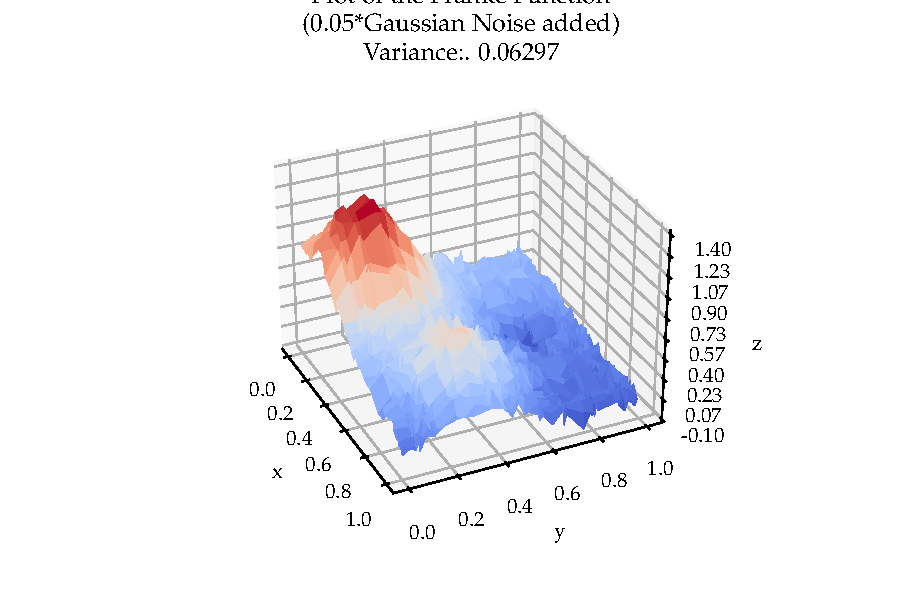
\includegraphics[scale=0.75]{figures/EX1_franke_function_noise_preview.pdf}
  \caption{\label{fig:2}Plot of the Franke Function with added stochastic noise}
\end{figure}

When constructing our OLS model, we start off by minimizing the cost function with regards to $\beta$. That is, we take the derivative of $C(\bm{X},\bm{\beta})$ and set it $0$. The following derivation shows how we end up with the optimal parameters $\bm{\hat{\beta}}$, which in turn can be used to predict new values for the function which we are fitting. 

\[
  \frac{\partial{C(\boldsymbol{X},\boldsymbol{\beta})}}{\partial{\beta}} = 0  
\]
\[
  \frac{\partial{C(\boldsymbol{X},\boldsymbol{\beta})}}{\partial{\beta}} = -\frac{2}{n}\bm{X}^\text{T}\left(\bm{y} - \bm{X}\bm{\beta}\right) = 0
\]
\[
  \bm{X}^\text{T}\left(\bm{y} - \bm{X}\bm{\beta}\right) = 0
\]
\[
  \bm{X}^\text{T}\bm{X}\bm{\beta} = \bm{X}^\text{T}\bm{y}
\]
\[
  \bm{\hat{\beta}} = \left(\bm{X}^\text{T}\bm{X}\right)^{-1}\bm{X}^\text{T}\bm{y}
\]
For consistency, it is noted that $\bm{\hat{\beta}} \in \mathbb{R}^p$, $\bm{y} \in \mathbb{R}^n$ and $\bm{X} \in \mathbb{R}^{n\times{p}}$.

With an expression for the predictors $\hat{\beta}$ derived, fitting a new value $\tilde{y}$ is simply $\tilde{y} = \bm{X}\bm{\hat{\beta}}$.

Our own implementation of Ordinary Least Square regression is implemented such that its use mimics that of SciKit-learn. \cite{scikit-learn} That is, we also include separate steps for initializing our model, fitting the model and predicting using the model using the just derived mathematical expression. For further inquiry about implementation, refer to the github repository linked in the \nameref{sec:A}.

\subsection*{Confidence Intervals}
Confidence intervals can be used to asses the uncertainty of a parameter. In our case, we will define confidence limits following the understanding of a Confidence Interval given in "Bootstrap Methods and their Application". That is, given a computed confidence region, any value inside the confidence region should be more likely than all values outside the confidence region. \cite{Davison1997}

Furthermore, when computing the confidence interval for the parameters $\beta$, we first compute the variance $\bm{\sigma^2}(\beta_j) = \bm{\sigma^2}\left[(\bm{X}\bm{X^\text{T}})^{-1}\right]_\text{jj}$. Where $\bm{X}\bm{X^\text{T}}$ is the Hessian matrix. Furthermore, it can be shown that the Hessian matrix can be given as the second derivative of the Cost function with respect to $\beta$. I.e. 
\[
  \frac{\partial^2C}{\partial{\bm{\beta^\text{T}}}\partial{\bm{\beta}}} = \frac{2}{n}\bm{X}\bm{X^\text{T}}
\]

\subsection*{Mean Squared Error and R2 score}
Two metrics that can be used to asses the quality of a model is its Mean Square Error (MSE) and R2 score. The MSE for any estimator is defined as 
\[
  \text{MSE}(\boldsymbol{y},\boldsymbol{\tilde{y}}) = \frac{1}{n}
  \sum_{i=0}^{n-1}(y_i-\tilde{y}_i)^2
\]
It will be shown later that the MSE can be broken into two components, namely the variance and the squared bias. As can be seen from the equation, the MSE would attain the value of 0 if $y_i = \tilde{y}_i$. Moreover, by rewriting the mean squared error as $\text{MSE} = \frac{1}{m}\left\lVert \bm{y} - \bm{\tilde{y}}\right\rVert_2^2$, it can be seen that the error increases as the Euclidean distance between the prediction targets increase. \cite{Goodfellow2016}

The R2 score (coefficient of determination) is another metric that can be related to how the model covers its own variance. Defined as, 
\[
  \text{R}^2(\boldsymbol{y}, \tilde{\boldsymbol{y}}) = 1 - \frac{\sum_{i=0}^{n - 1} (y_i - \tilde{y}_i)^2}{\sum_{i=0}^{n - 1} (y_i - \bar{y})^2}
\] the closer the R2 score is to its maximum value 1, the more the variance of the model is explained by the model parameters. The R2 score gives a measure of model skill as a higher R2 generally indicates that the model is better at making new predictions. However, a perfect R2 score of 1 would result in the model covering it's entire variance, thus the model is overfitted and will not perform well in a general use case beyond the scope of it's initial training-data.

\textbf{TODO} Possibly more one implementation

\subsection*{Some words on Scaling}
Our motivation for scaling the data arise in the context of fitting a design matrix of predictors with different units. To avoid having to disregard some predictors in favor of others based on their unit, not necessarily their contribution to the function fit, a scaling of the data is performed. By scaling the data using one of several scaling techniques, we ensure that all predictors lie in the same reference domain, resulting in a more accurate representation of the predictors. SciKit-learn includes several different Scalers, such as the StandardScaler and MinMaxScaler. \cite{scikit-learn} For this discussion, the StandardScaler will be inspected.

The idea behind scaling the data with regards to the StandardScaler method, is to subtract the mean value for each column from the same column in the design matrix. This process is what is known as zero centering. Moreover, when scaling in this way, the intercept will be scaled by the mean value of the output. Moreover, it can be shown that zero centering leads to the new $\bm{\tilde{y}} = \bm{y} - \beta_0 = \bm{y} - \bm{\bar{y}}$, where $\bm{\bar{y}}$ is used as the sample mean of $\bm{y}$. As the columns of $\bm{X}$ also has been scaled in the same fashion, we end up the following Cost-Function
\[
  C(\boldsymbol{\beta}) = (\boldsymbol{\tilde{y}} - \tilde{X}\boldsymbol{\beta})^T(\boldsymbol{\tilde{y}} - \tilde{X}\boldsymbol{\beta}).  
\]

Before scaling the dataset, an assessment of how to deal with the intercept has to be made. For reference, the intercept is defined as the first column of the design matrix, and for a polynomial fit would represent where the function intercepts with the y-axis when all other features are set to zero. Moreover, the intercept is a constant value (1), thus zero centering the intercept would result in a singular matrix, rendering the optimization problem unsolvable. Throughout this assignment, we are going to readd the intercept after scaling, essentially leaving the intercept untouched as to avoid any singular matrices. Moreover, for ordinary least squares regression, as there is no regularization of the predictors during the model fit, a model fitted on scaled contra unscaled data would attain the same mean squared error.

However, other regression methods such as Ridge and Lasso, which will be discussed in greater detail in further sections, have a dependance on the intercept through the hyperparamter $\lambda$ when computing their regularization term. Not including the intercept when computing the regularization term would give rise to a divergence between the mean square error for the model scaled with compared to the model scaled without the intercept. Thus, by computing the regularization term with disregard to the intercept, the first $\beta_j$ i.e. that of the intercept will be skipped in the computation. This will in most cases lead to a better mean square error for both Ridge and Lasso regression. Skipping the intercept when computing the regularization term also follows the definition of Ridge regression as in. \cite{Geron2019}

Furthermore, while on the topic of Ridge and Lasso regression, scaling of the data should always be performed. This is due to the regularized linear models such as Ridge and Lasso being sensitive to the scale of the input features. \cite{Geron2019}

To determine whether scaling is apropriate for the current problem, that being fitting the Franke Function using oridnary least squares, an inspection of the generated data is made in light of the just discussion. For Exercise 1, the datapoints $x,y \in \left[0,1\right]$. This would indicate that the data is already scaled to a unit reference system. Moreover, as we are training a model based on the ordinary least squares, there is no dependance on scale of the input features as for regularized linear models. However, for consistency with further models, the data will be scaled with respect to the training data. However, the target variables however will not be scaled.

\subsubsection*{Splitting the data}
As we want our model to perform well in general cases, we split the data into a training and testing set to simulate model prediction using new data. This is achieved by the aforementioned split, since the training and test data are kept entirely separated. In practice, we fit the model using the training data, then perform a test of the model using the test data. The error rate for new cases predicted by the model using the test data, can be used to understand how the model will perform on new untrained data. \cite{Geron2019} Moreover, by assessing the deviation between training error and test error, it can be seen whether the model is overfitting or not. It would be a case of overfitting if the training error is low, whereas the test error is high.

Throughout this assignment, we will split the data into a train and test set. The data could be split into an additional validation set, which is normally used for hyperparamter adjustment. However, as we don't see any practical use for a validation set for this assignment, we will skip out on splitting the data into an additional validation set. Though a validation set could be used for tuning the hyperparameter to select an optimal model, it could also lead to suboptimal model selection caused by imprecise prediction from a too small validation set. \cite{Geron2019} Though our data consists of potentially unlimited data points, due to computational time constraints, we will resort to a relatively sparse dataset. Hence, we split into a training and test set to avoid sacrificing the training data in favor of a sufficient validation set.

Had we not omitted the validation set for hyperparameter tuning, the process of studying regularized models would have deviated somewhat from the study of the ordinary least squares regression. The process would then be that we split the data into a train-test split, as before. Moreover, the training data would have been split once more into a train and validation set, with an approximate ratio of 80 - 20 percent respectively. Furthermore, the hyperparameters are tuned with the MSE obtained from predicting using the validation set. However, as the validation set typically reports a lower error than the test set, the generalization error of the optimized model is studied using the test set. \cite{Goodfellow2016}

\subsection*{Comparing our OLS implementation to the one delivered by SciKit-learn}
With our Ordinary Least Squares model implemented as described above, we start off by benchmarking our implementation to the LeastSquares method found in SciKit-learn. \cite{scikit-learn} We start off by setting up a uniform 2-dimensional grid and initialize a Franke Function with some added stochastic noise.

\begin{lstlisting}
  np.random.seed(4155)
  n = 100
  x = np.sort(np.random.uniform(0, 1, n))
  y = np.sort(np.random.uniform(0, 1, n))
  x, y = np.meshgrid(x,y)
  z = FrankeFunction(x, y) 
  noise = 0.5 * np.random.randn(n,n)
  z += noise
\end{lstlisting}

For this initial run, we are interested in studying the least squares fit of the Franke Function up to the fifth order. 

\begin{figure}[h]
  \centering
  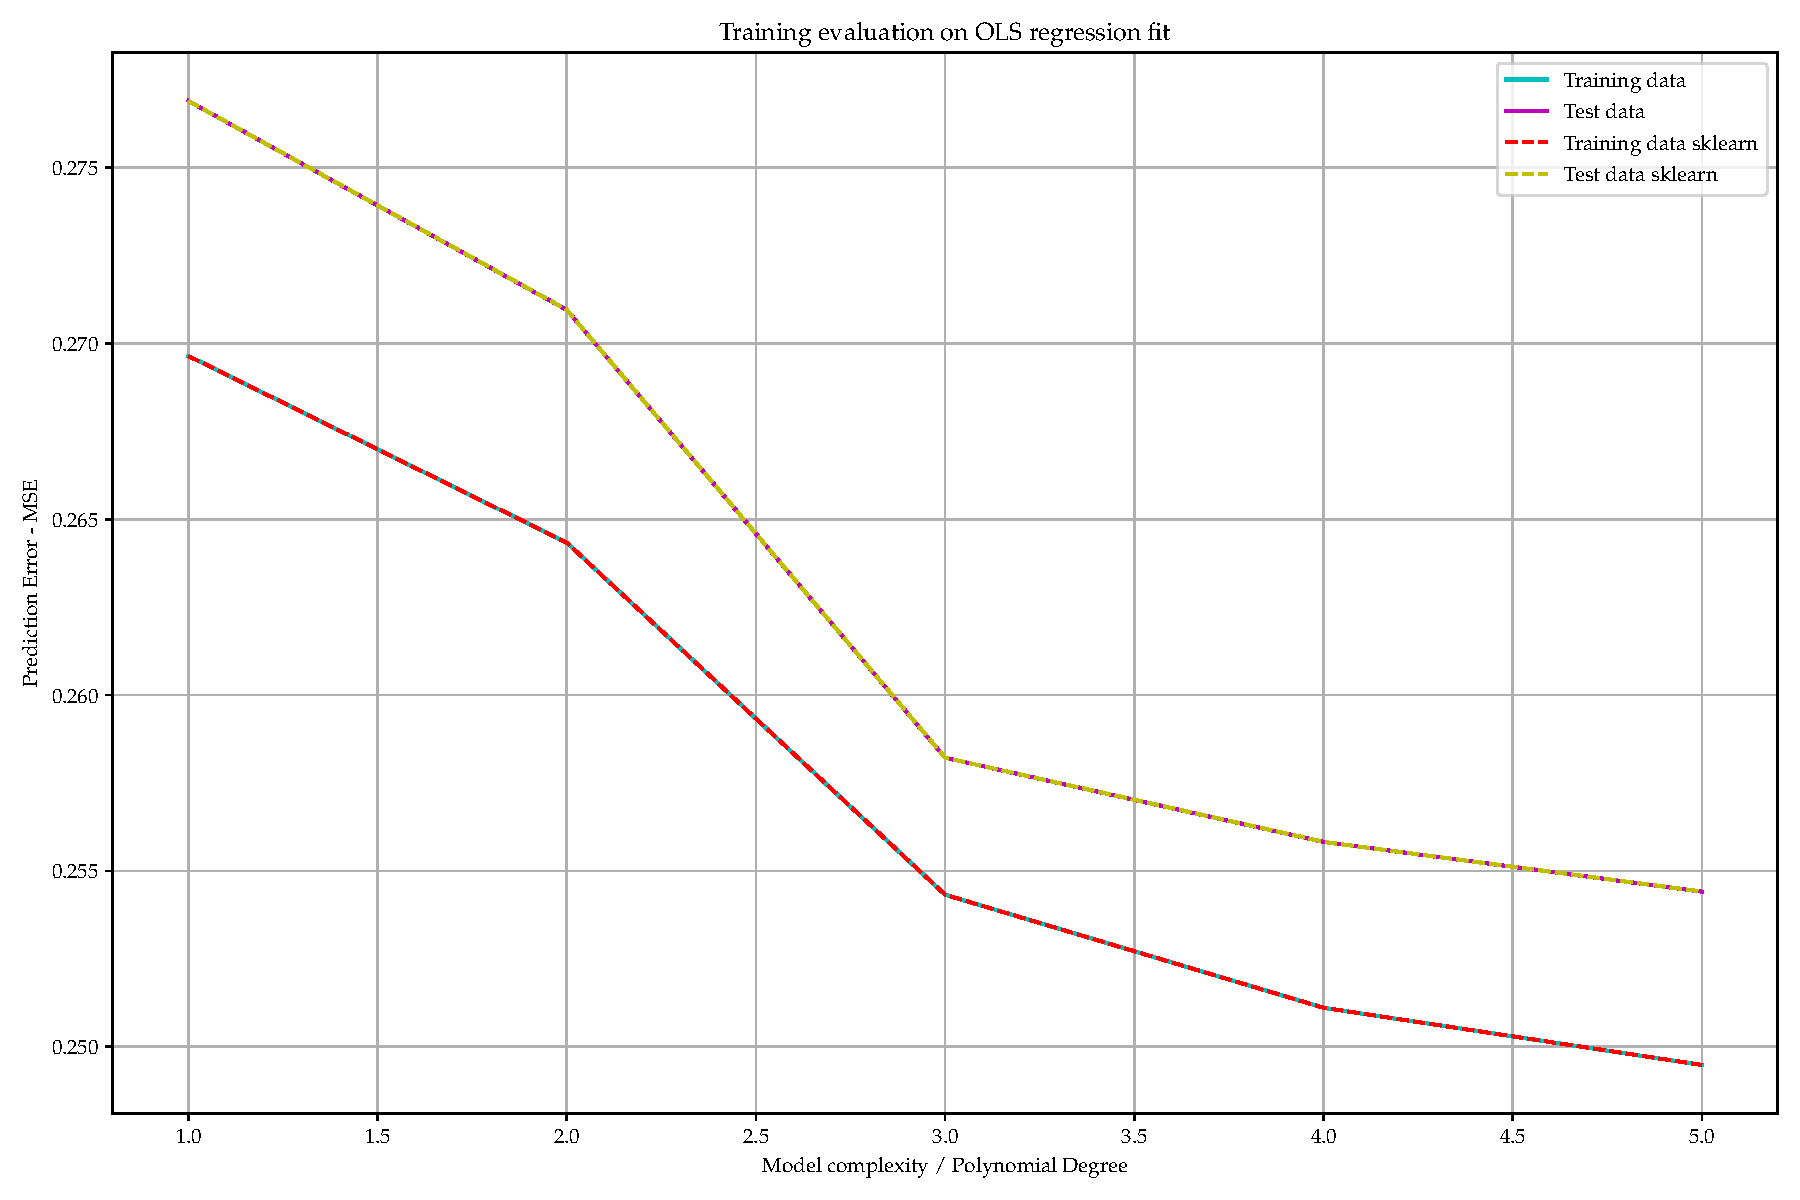
\includegraphics[scale=0.5]{figures/EX1_franke_function_OLS_evaluate_fit_1.pdf}
  \caption{\label{fig:OLS_franke_1} Benchmark run with degree up to the fifth order of our OLS implementation compared to the similar LinearRegression() from SciKit-learn}
\end{figure}

By inspecting Figure (\ref{fig:OLS_franke_1}), we can see that there are no visual differences between our implementation of OLS compared to the SciKit-learn implementation. Moreover, there seem to a reduction in MSE as model complexity increases. The Confidence Interval for the predictors $\beta_j$ is constructed for the fit using up to fifth order polynomials. As the predictors are based not only of the x and y parameters in isolation, but also their interaction terms, a fifth order fitted model includes 21 different predictors. The result of computing the Confidence Interval for the 21 different predictors can be seen in Figure \ref{fig:OLS_beta_1}. Note that the predictors  From Figure \ref{fig:OLS_beta_1}, it can be seen that the lowermost and higher order terms have the smallest confidence intervals. Leaving the predictors of order 3 and 4 with a higher uncertainty.

\begin{figure}
  \centering
  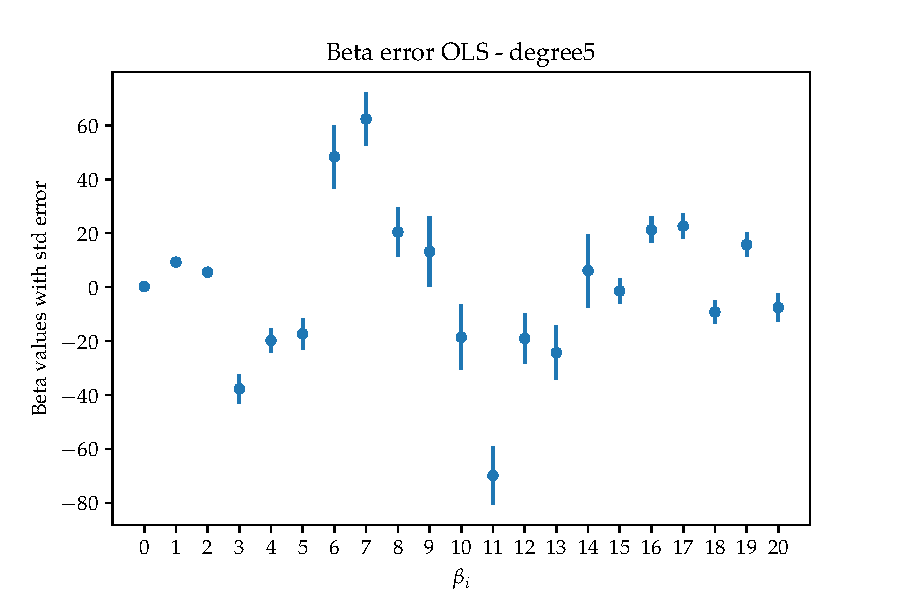
\includegraphics[scale=.85]{figures/EX1_OLS_beta_error_degree5.pdf}
  \caption{\label{fig:OLS_beta_1} 95\% Confidence intervals for the predictors of an OLS model with polynomials up to the fifth order.}
\end{figure}

%\begin{figure}
%  \centering
%  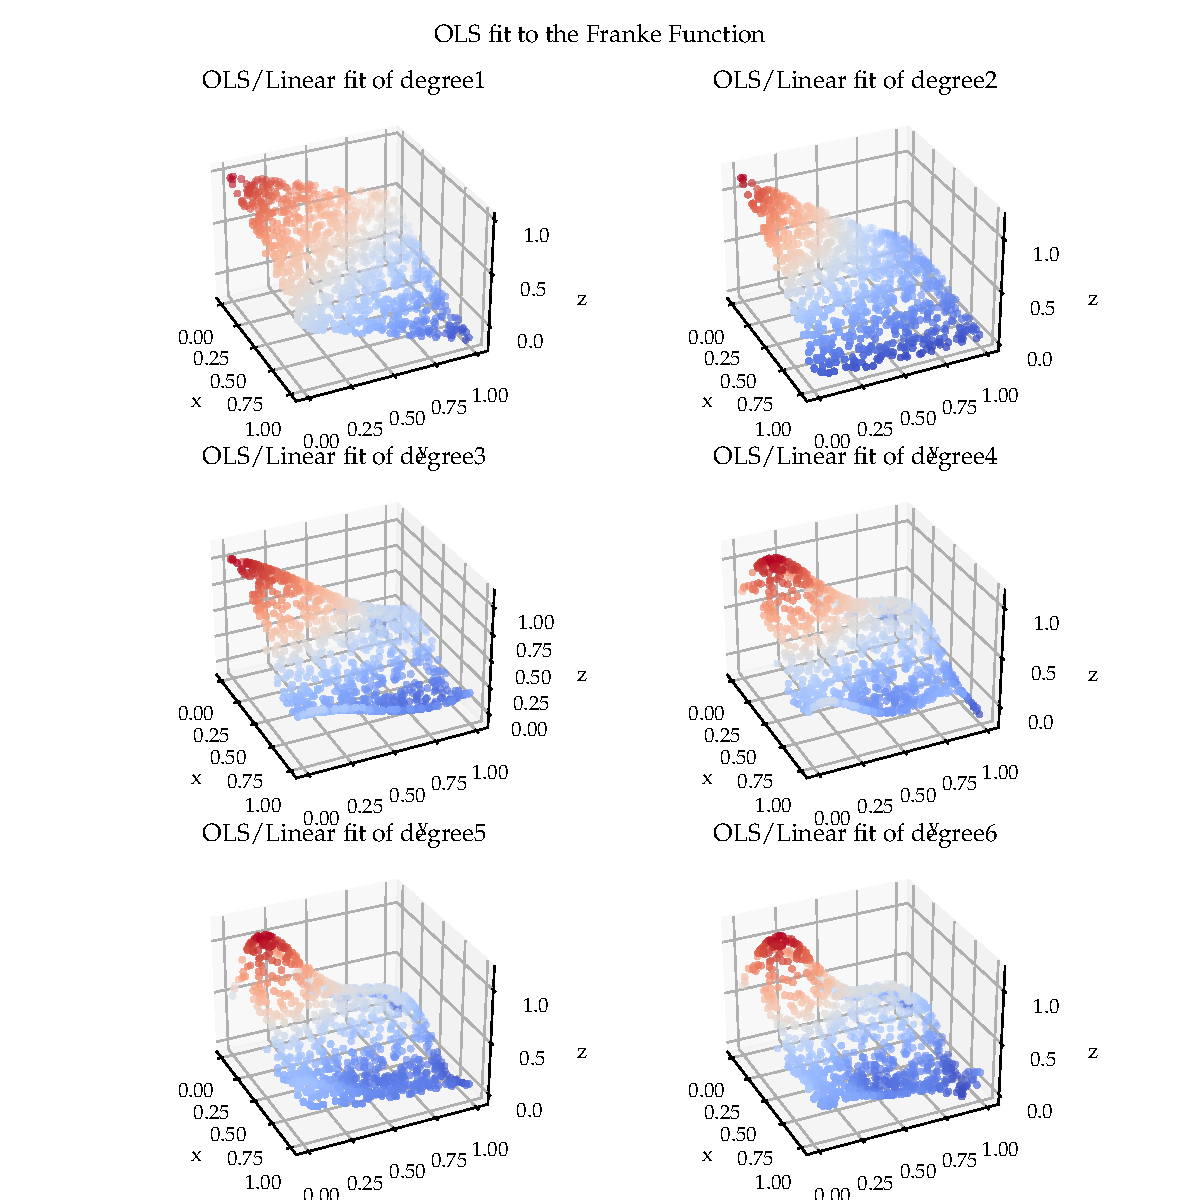
\includegraphics[scale=0.85]{figures/franke_function_OLS_fit.pdf}
%  \caption{?}
%  \label{fig:3}
%\end{figure}

%\begin{figure}
%  \centering
%  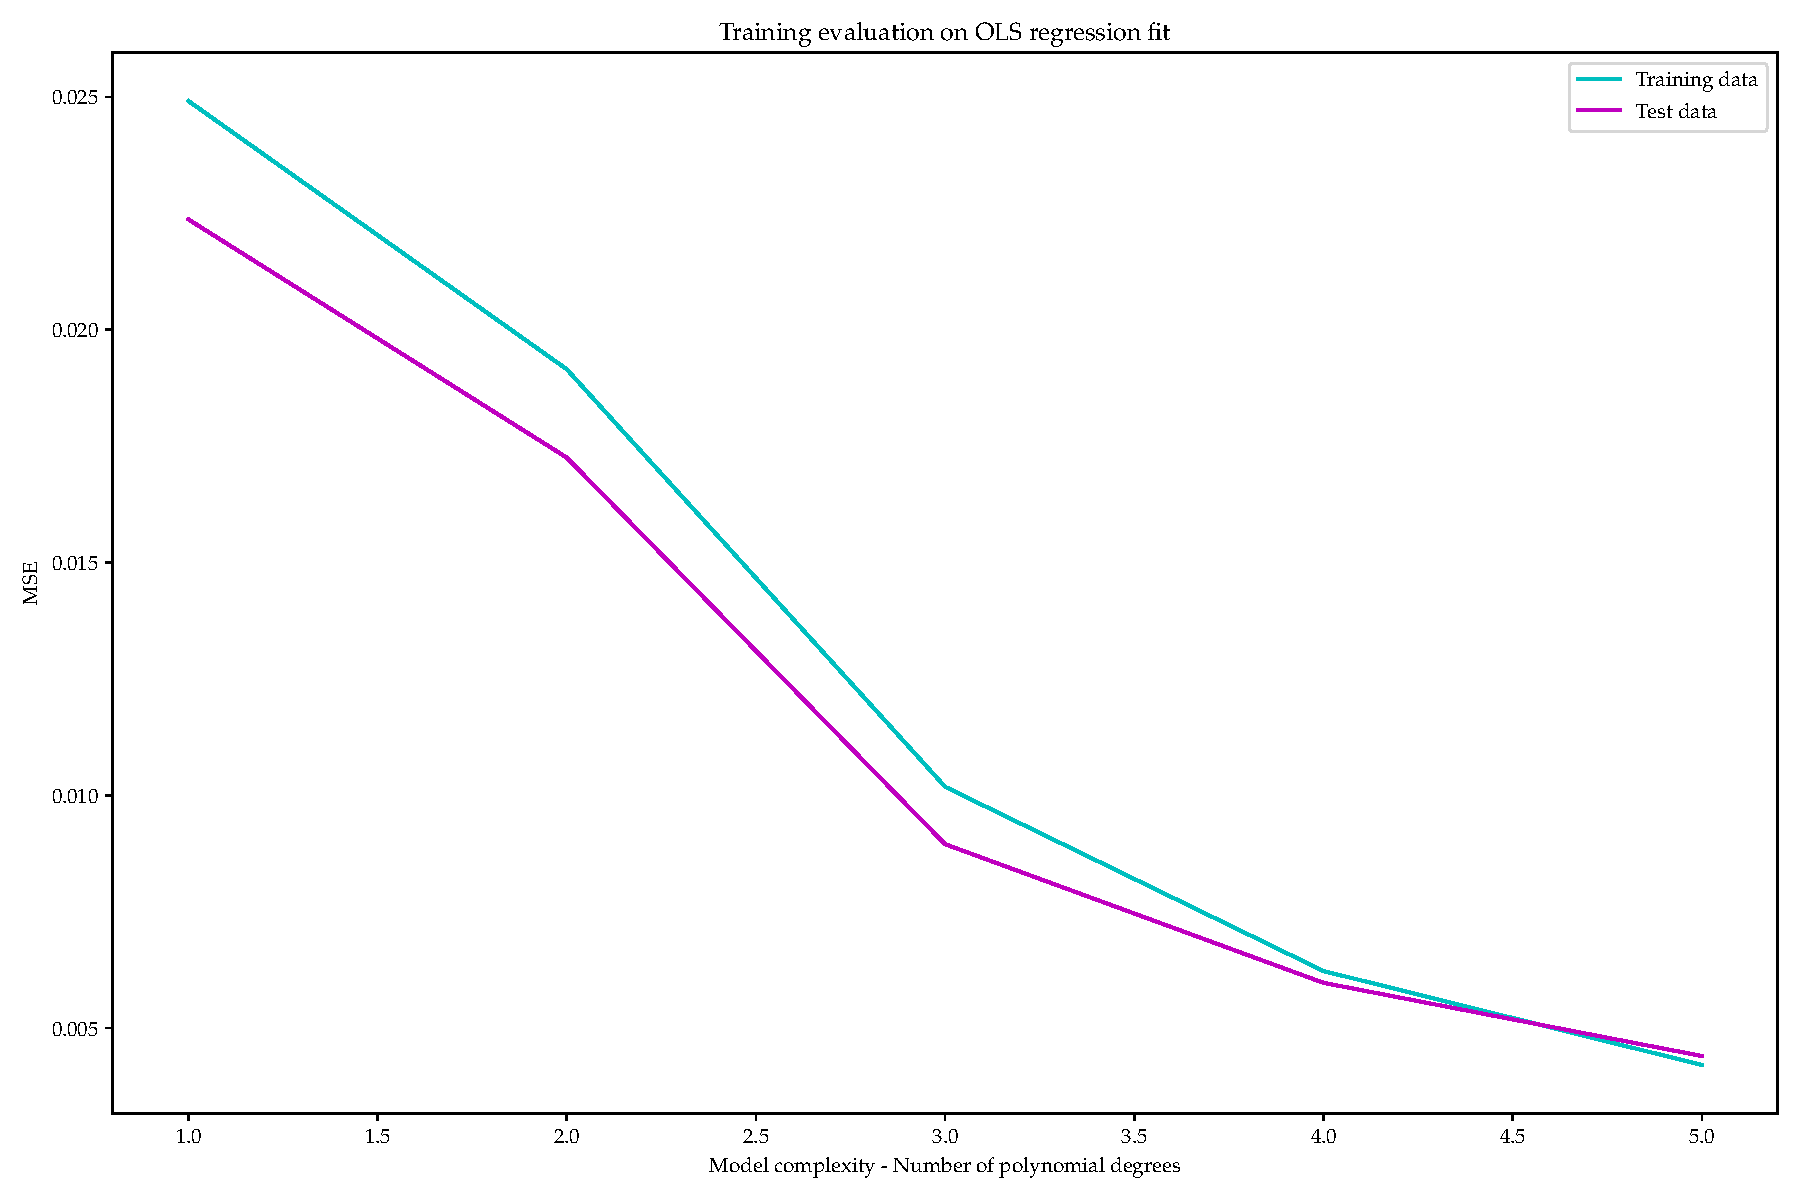
\includegraphics[scale=0.45]{figures/franke_function_OLS_evaluate_fit.pdf}
%  \caption{?}
%  \label{fig:4}
%\end{figure}

%\begin{figure}
%  \centering
%  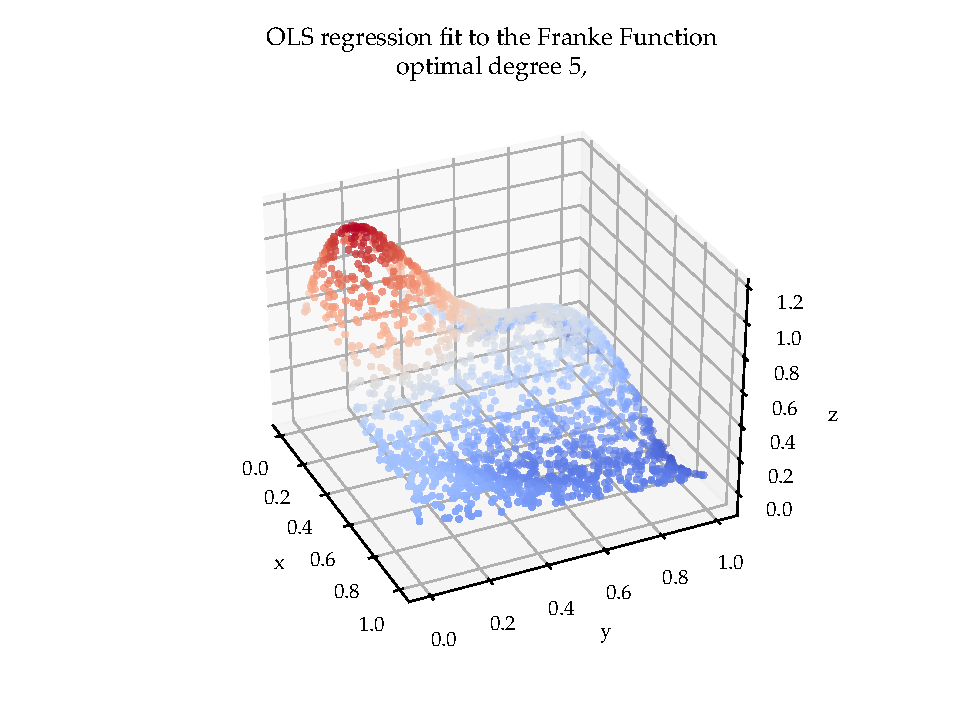
\includegraphics[scale=0.85]{figures/franke_function_OLS_best_fit.pdf}
%  \caption{?}
%  \label{fig:5}
%\end{figure}


\section*{Exercise 2}
\subsection*{Some words on bootstrapping}


Moving on to the bias-variance trade-off analysis, we start off by showing that 

\[
  C(\bm{X},\bm{\beta}) =\frac{1}{n}\sum_{i=0}^{n-1}(y_i-\tilde{y}_i)^2=\mathbb{E}\left[(\bm{y}-\bm{\tilde{y}})^2\right]
\]

Can be rewritten as

\[
\mathbb{E}\left[(\bm{y}-\bm{\tilde{y}})^2\right]=\frac{1}{n}\sum_i(f_i-\mathbb{E}\left[\bm{\tilde{y}}\right])^2+\frac{1}{n}\sum_i(\tilde{y}_i-\mathbb{E}\left[\bm{\tilde{y}}\right])^2+\sigma^2.
\]

where the terms are respectively $(\text{bias})^2$, variance and noise. For simplicity, assume that we have a dataset where the data is generated from a noisy model

\[\bm{y} = f(\bm{x}) + \bm{\epsilon}\]

Furthermore, we will assume that the residuals $\epsilon$ are independant and normally distributed $\epsilon \sim \mathcal{N}(0, \sigma^2)$. Finally, $\bm{\tilde{y}} = \bm{X}\bm{\beta}$ is our approximation to the functions $f$. Start off by adding and subtracting $\mathbb{E}\left[\bm{\tilde{y}}\right]$ inside the expectation value.

\[
  \mathbb{E}\left[(\bm{y}-\bm{\tilde{y}})^2\right] 
  = \mathbb{E}\left[(\bm{y}-\bm{\tilde{y}} + \mathbb{E}\left[\bm{\tilde{y}}\right] - \mathbb{E}\left[\bm{\tilde{y}}\right])^2\right] 
\]
\[
  = \mathbb{E}\left[((\bm{y} - \mathbb{E}\left[\bm{\tilde{y}}\right]) - (\bm{\tilde{y}} - \mathbb{E}\left[\bm{\tilde{y}}\right]))^2\right]
\]
By using the fact that $\bm{y} = f(\bm{x}) + \bm{\epsilon}$
we can rewrite this as
\[
  = \mathbb{E}\left[((f(\bm{x}) - \mathbb{E}\left[\bm{\tilde{y}}\right]) - (\bm{\tilde{y}} - \mathbb{E}\left[\bm{\tilde{y}}\right]) + \epsilon)^2\right]
\]
Computing the square inside the expectation value gives us
\[
  = \mathbb{E}\left[(f(\bm{x}) - \mathbb{E}\left[\bm{\tilde{y}}\right])^2 + (\bm{\tilde{y}} - \mathbb{E}\left[\bm{\tilde{y}}\right])^2 + \epsilon^2 \right]\]
  \[+ 2\left(\mathbb{E}\left[\epsilon(f(\bm{x}) - \mathbb{E}\left[\bm{\tilde{y}}\right])\right]- \mathbb{E}\left[\epsilon(\bm{\tilde{y}} - \mathbb{E}\left[\bm{\tilde{y}}\right])\right] - \mathbb{E}\left[(f(\bm{x}) - \mathbb{E}\left[\bm{\tilde{y}}\right])(\bm{\tilde{y}} - \mathbb{E}\left[\bm{\tilde{y}}\right])\right]\right)
\]
Moreover, as $\epsilon$ are independant variables, the expectation value involving them as a product can be written as a product of expectation values. Knowing that $\mathbb{E}\left[\epsilon\right] = 0$, the third and second to last term is equal to zero. Also, knowing that $\mathbb{E}\left[\bm{\tilde{y}}\right] = \bm{\tilde{y}}$, the last t

\begin{equation}\label{eq:varbi}
  = \mathbb{E}\left[(f(\bm{x}) - \mathbb{E}\left[\bm{\tilde{y}}\right])^2\right] + \mathbb{E}\left[(\bm{\tilde{y}} - \mathbb{E}\left[\bm{\tilde{y}}\right])^2\right] + \mathbb{E}\left[\epsilon^2 \right]
\end{equation}
The first term in (\ref{eq:varbi}) can be discretized as
\[
  \mathbb{E}\left[(f(\bm{x}) - \mathbb{E}\left[\bm{\tilde{y}}\right])^2\right] = \frac{1}{n}\sum_i(f_i - \mathbb{E}\left[\bm{\tilde{y}}\right])^2
\]
Which is the bias squared as we were to show.

The second term in (\ref{eq:varbi}) is also discretized, yielding
\[
  \mathbb{E}\left[(\bm{\tilde{y}} - \mathbb{E}\left[\bm{\tilde{y}}\right])^2\right] = \frac{1}{n}\sum_i(\bm{\tilde{y}} - \mathbb{E}\left[\bm{\tilde{y}}\right])^2
\]
Which takes form of the variance, as was set out to show.

Finally, it can be shown that $\text{var}(\bm{y}) = \text{var}(f + \epsilon) = \mathbb{E}\left[(f + \epsilon)^2\right] - (\mathbb{E}\left[(f + \epsilon)\right])^2$ = $\mathbb{E}\left[\epsilon^2\right]$ As such, we can use that \[
  \text{var}(y) = \sigma^2 = \mathbb{E}\left[\epsilon^2\right]
\]
to see that the final term in (\ref{eq:varbi}) is equal to the noise. Thus we have shown that 
\[
\mathbb{E}\left[(\bm{y}-\bm{\tilde{y}})^2\right] = \mathbb{E}\left[(f(\bm{x}) - \mathbb{E}\left[\bm{\tilde{y}}\right])^2\right] + \mathbb{E}\left[(\bm{\tilde{y}} - \mathbb{E}\left[\bm{\tilde{y}}\right])^2\right] + \mathbb{E}\left[\epsilon^2 \right]
\]
\[
=\frac{1}{n}\sum_i(f_i-\mathbb{E}\left[\bm{\tilde{y}}\right])^2+\frac{1}{n}\sum_i(\tilde{y}_i-\mathbb{E}\left[\bm{\tilde{y}}\right])^2+\sigma^2.
\]

The final expression consists of three terms. The first term is a sum of the squared bias, the second term is the variance and the final term is a constant noise term. The sum of squared bias and variance make up the mean square error of our model. \cite{Hastie2009} 

The bias component of the mean square error measures the difference from the true mean to the desired regression model. As function of model complexity, the bias will decrease as complexity increases. The second term, the variance, gives a measurement of the variation of the model values around their average value. The variance will increase with model complexity. The constant noise term $\sigma^2$ is an irreducible error, and as such does not contribute when analysing the bias-variance tradeoff.

The bias-variance tradeoff can be used as a method for model selection. As has been alluded to in the previous paragraph, the variance is inverse proportional to the bias. As such, there is a trade-off between bias and variance. As the bias-variance is directly related to the mean square error for both the training data but also test and production data used for making new predictions. When selecting a model we wish to balance and minimize both quantities, as that leads to the model with the best predicitve capabilities. \cite{Bishop2016}

Furthermore, the problem of overfitting can also be discussed in light of the bias variance tradeoff. Overfitting is proportional to the model variance, as such a high variance leads to an overfitted model. An overfitted model is one that has learned the noise of the training data, resulting in a perfect fit for the training data but a high mean square error when predicting using new data. Hence, a higher bias can be considered more useful to circumvent overfitting.

Lastly, it should be noted that the bias-variance tradeoff measuremnet is performed for a single dataset of limited size. As such, if there were more datapoints to train the model with, the model would attain a better overall fit. Moreover, a greater amount of training data would reduce the level of overfitting for a given model complexity. \cite{Bishop2016} Though there are some limitations to the measurement, the bias-variance tradeoff can be used to estimate where the trained model is general enough to both avoid under -and overfitting (i.e. too high bias or too high variance).

%\begin{figure}
%  \centering
%  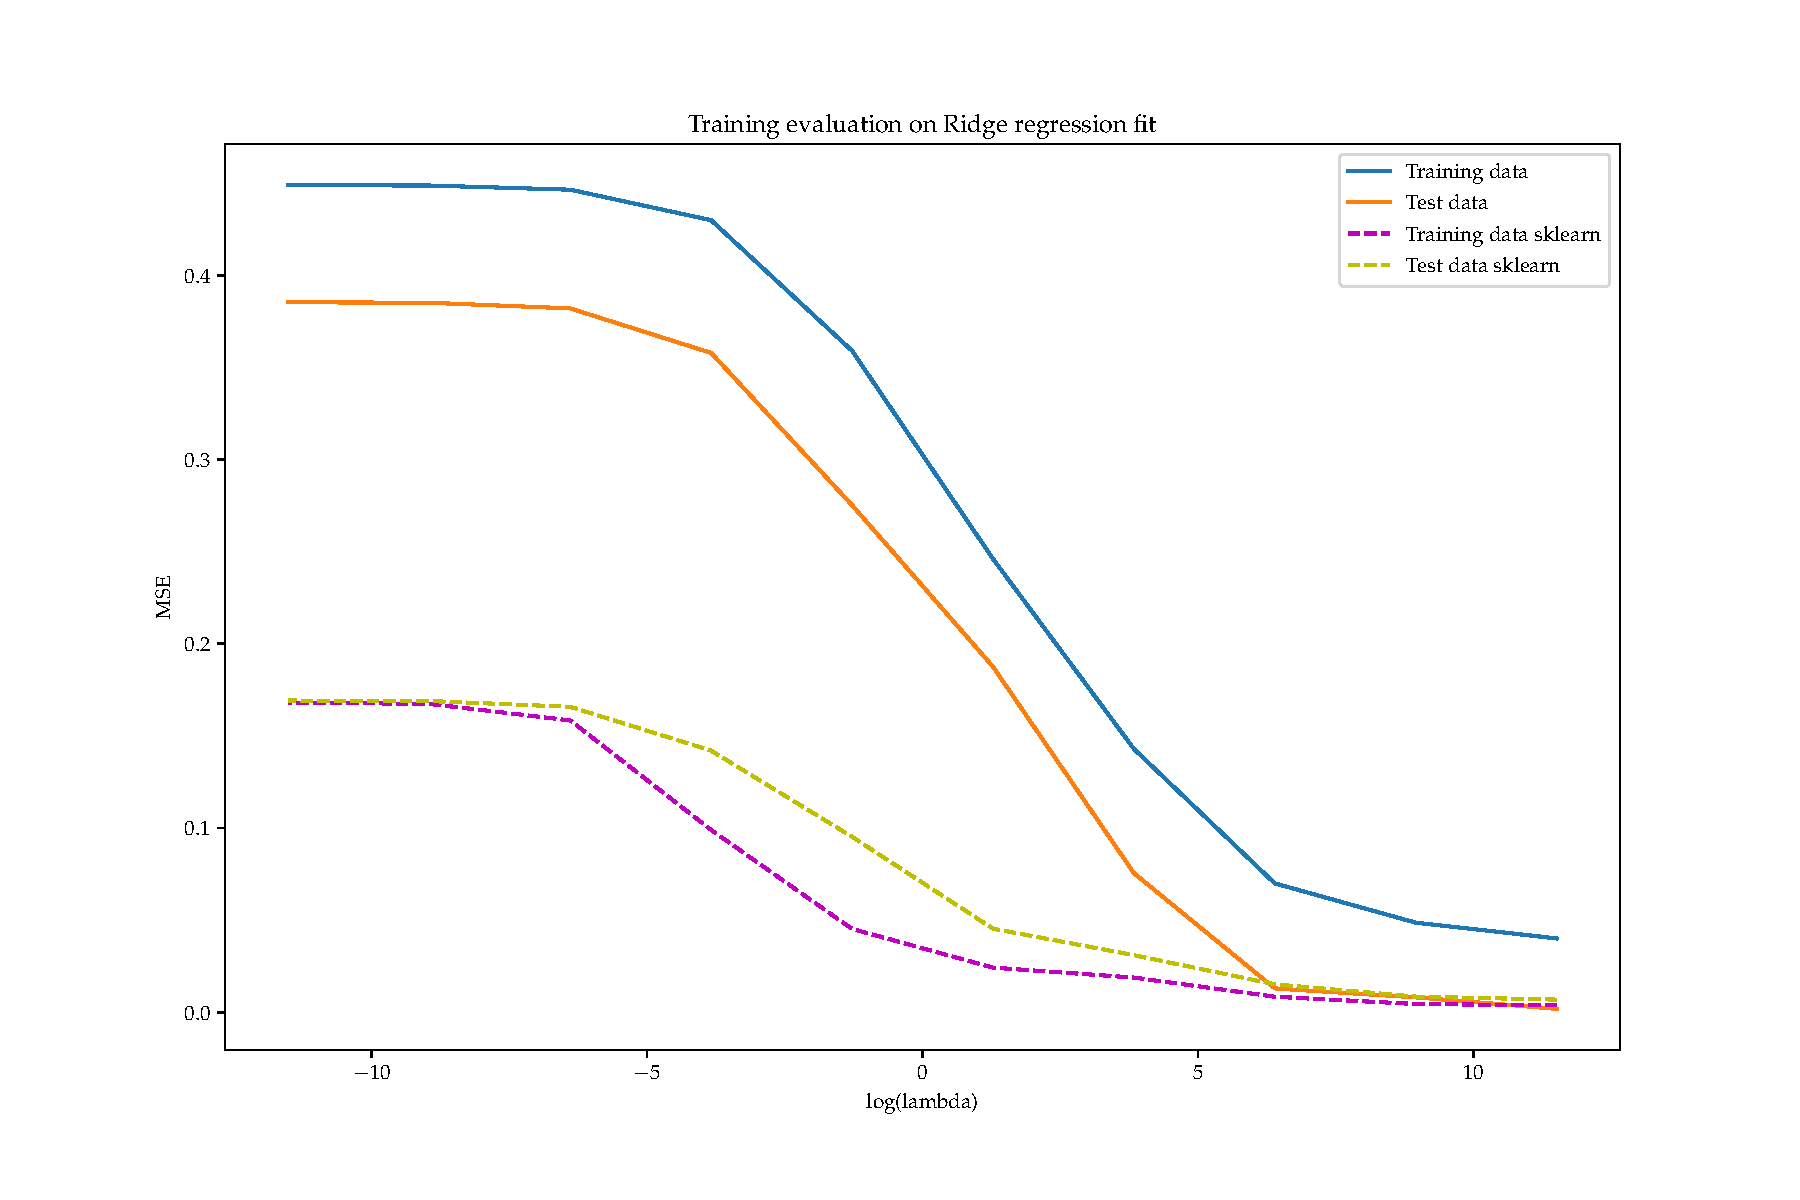
\includegraphics[scale=0.45]{figures/franke_function_Ridge_evaluate_fit.pdf}
%  \caption{The best fit using Ridge}
%  \label{fig: Ridge_best_fit}
%\end{figure}

%\begin{figure}
%  \centering
%  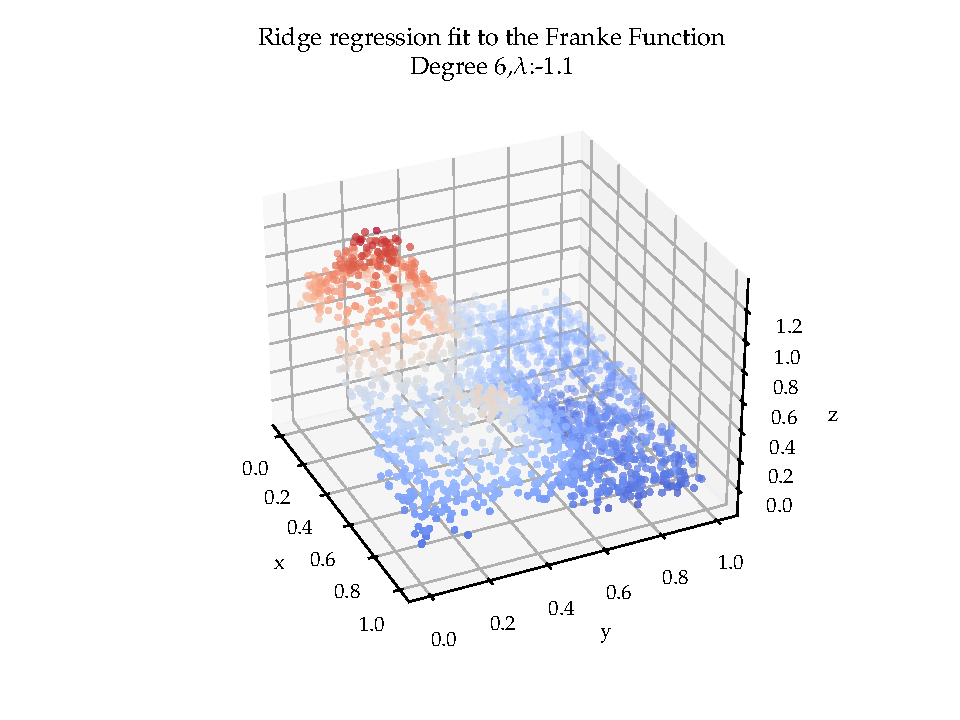
\includegraphics[scale=0.85]{figures/franke_function_Ridge_best_fit.pdf}
%  \caption{The best fit using Ridge}
%  \label{fig: Ridge_best_fit_2}
%\end{figure}

\begin{center}
  \csvautobooktabular{data/report_data/redge_reg_lambda_-1.1.csv}
  \label{data: Ridge_best_fit}
\end{center}


\section*{Appendix\label{sec:A}}
\textbf{TODO} her skal det ligge link til et github repo. 

\newpage
\newpage

\bibliographystyle{plain}
\bibliography{bibliography}




\end{document}


% Local Variables:
% TeX-engine: xetex
% End:
